\chapter{Constitution du corpus}

\section{Une histoire des corpus latins numériques}

Le travail sur la langue latine nécessite \textit{de facto} des corpus, et \textit{a priori} en nécessite des numériques s'il s'agit d'une approche computationnelle. Si la tradition papier des corpus académiques des Teubner ou des Belles Lettres s'inscrira bientôt dans leur troisième centenaire\footnote{Si l'éditeur Teubner semble s'attaquer dès les années 1810 à l'impression d'ouvrages philologiques, la \textit{Bibliotheca Scriptorum Graecorum et Latinorum Teubneriana} ne voit le jour \enquote{qu'en} 1849. Elle prédate les deux autres collections généralistes majeurs, la collection \textit{Oxford Classical Texts} et les \textit{Belles Lettres}. \cite{andre_cent-cinquante_1974}}, l'histoire des corpus littéraires numériques n'a fêté que très récemment son cinquantenaire avec les prémices du \textit{Thesaurus Linguae Graecae}.

Aussi, nous proposons de revenir sur les cinquante dernières années de numérisation et de mise à disposition des textes latins, principalement des textes littéraires. Nous proposons un découpage en trois périodes de cette révolution numérique des corpus: la première concerne l'apparition des disquettes et CD de corpus qui émaille les décennies 1960 à 1990; la seconde (1995-2005) concerne l'apparition en ligne de ces premiers corpus, mais aussi une autre forme de révolution, celle des corpus non académiques; la troisième (2005-aujourd'hui) concerne enfin l'expansion du numérique comme version fondamentale des corpus et l'apparition de \enquote{méga corpus}.

Il faudra cependant commencer cette introduction au chapitre par un avertissement: la documentation disponible sur la publication des corpus numériques est presque inexistante, souvent de seconde main, à travers de rares témoignages ou d'encore plus rares citations et ne permet souvent pas de retrouver avec toute l'exactitude souhaitée la première date de publication de tel ou tel ouvrage. Jusqu'à aujourd'hui, la citation des corpus numériques n'est pas entrée dans les usages, tout comme la citation des oeuvres quand on en fait le commentaire: rares sont les chercheurs qui spécifient en bibliographie l'édition précise qu'ils ont utilisée quand ils mentionnent Virgile ou Martial. Aussi, nous nous excusons d'avance  si des informations présentées ici sont inexactes, si des corpus oubliés le sont, et nous invitons grandement notre champ à capturer rapidement cette histoire, l'archiver avant qu'il ne soit trop tard: si les décades 70 et 80 ne sont pas très loin, elles semblent bien floues sur le plan de l'histoire des corpus\footnote{Il nous semble propice, pour qui voudra, de s'intéresser à une histoire orale des projets fondateurs, à une recherche en archives pour chacun de ces projets, avant qu'il ne soit trop tard.}.

\subsection{Les \enquote{incunables} du numérique}

Nous nous intéressons ici à la naissance des corpus numériques littéraires, ayant pour vocation d'être lus ou utilisés pour des recherches dès leur conception numérique. À cette fin, nous excluons les travaux d'annotation linguistique et de construction de concordanciers de R. Busa ou du LASLA  car ils avaient des ambitions plus spécifiques et ne proposaient pas comme but premier de pouvoir lire le texte\footnote{Mais nous en parlerons plus tard, \textit{cf.} \ref{lemmatisation:concordanciers}}. Or, il est difficile comme nous le disions plus haut de savoir à quand remontent les premières productions de corpus.

% La documentation d’époque et de première main est très pauvre sur ces outils (date, recherche en cours), on les retrouve principalement dans des reviews

\subsubsection{Années 60, années 80: premiers corpus, premiers CD-ROMs}

Le corpus littéraire le plus ancien dont il est fait mention est celui financé par le \textit{National Endowment for the Humanities} (NEH) et cité par Theodore F. Brunner dans son article rétrospectif de 1993 centré sur la recherche états-unienne \textit{Classics and the Computer}\footcite{brunner_classics_1993}. En 1968, Nathan Greenberg et John. J. Bateman obtiennent un financement de la NEH de 19.800\$ \footcite{noauthor_neh_2018} complété par 40.000\$ de financeurs secondaires, dont IBM\footnote{D'après \cite{brunner_classics_1993}: le \textit{Digital Computer Laboratory} de l'université d'Illinois, the \textit{Kiewit Computation Center} du Dartmouth College, la \textit{National Science Foundation}, la fondation Ford et l'entreprise IBM donc.}. Avec ce dernier, ils organisent une école d'été titrée \textit{Summer Institute in Computer Applications to Classical Studies}\footnote{L'équivalent de 59~800\$ au 31 janvier 1968 est de 479~745\$ en août 2021 d'après le calculateur d'inflation du \textit{Bureau of Labor Statistics}, \cite{noauthor_cpi_nodate})}. Cet événement donne naissance à un corpus d'une vingtaine d'oeuvres grecques et latines plus ou moins complètes: on y trouve à côté des classiques homériques des morceaux d'oeuvres, parfois inattendus, dont la découpe est particulière, tel le poème 64 de Catulle qui est édité seul, trois oeuvres de l'\textit{Appendix Vergiliana}, les livres I, IV, IX et XII de l'\textit{Énéide}. En dehors d'un rapport, ce corpus ne semble pas avoir eu une vie particulièrement riche, ni de nom d'ailleurs: il est pris en charge par l'\textit{American Philological Association}, est dupliqué à la demande par des institutions, mais très vite se voit couper de tous fonds supplémentaires, là où, comme le note 20 ans plus tard Brunner, le fond des monographies n'est pas touché\footcite{brunner_classics_1993}.

Au début des années 70, nous trouvons la trace d'un seul autre corpus, celui du \textit{Thesaurus Linguae Grecae} (TLG) dont les prémices remontent à 1971\footcite{brunner_classics_1993} et dont la naissance est actée en 1973\footnote{Parmi les articles cités par T. F. Brunner lui-même sur la fondation du TLG, au moins un est indisponible en France: \cite{Hughes_homer_1987}}. Si son nom est dérivé d'un projet humaniste du 16\textsuperscript{e} siècle et est en écho à celui du dictionnaire \textit{Thesaurus Linguae Latinae} (TLL), il ne s'agit que d'une simple inscription dans une tradition des grands travaux humanistes: à contrario des deux derniers, ce projet se veut dès les premières conférences un corpus de texte et non un thésaurus, un dictionnaire fortement enrichi. Les premières versions du corpus voient rapidement le jour pour atteindre 61 millions de mots en 1988\footcite{brunner_overcoming_1988}, via une externalisation de la copie \enquote{manuelle} des volumes en Corée du Sud (1972-1980) puis aux Philippines\footcite[p. 111]{helgerson_cd-rom_1988}. Ce corpus pose une difficulté de taille, à savoir son alphabet: en 1972, seuls les caractères ASCII\footnote{\textit{American Standard Code for Information Interchange}} existent informatiquement, ils sont au nombre de 128 et couvrent les nombres, les caractères latins hors diacritiques et les signes de ponctuation. Il faut trouver une solution pour les caractères grecs, et c'est un certain David W. Packard qui trouve une méthode pour encoder ces derniers, le BetaCode. Cette méthode de transcription, dont il reste des traces encore aujourd'hui dans des fichiers de Perseus, propose l'encodage des diacritiques via les signes de ponctuation: ainsi, la parenthèse \texttt{)} remplace l'esprit doux, tandis que le pipe \texttt{|} représente le iota souscrit, par exemple, \textgreek{αναλαβόντες δὲ καθ᾽ ἕκαστον} donne \texttt{analabo/ntes de\ kaq`e(/kaston.}


Présent à la réunion de fondation du projet TLG et résolveur du problème d'encodage, David W. Packard n'est pas seulement important pour ce dernier: il fonde le Packard Humanities Institute (PHI) en 1987\footcite{helgerson_cd-rom_1988}, institut ayant pour visée de produire des corpus, dont un équivalent latin du TLG\footnote{Le corpus latin n'est qu'un des multiples corpus du PHI, même si l'on utilise souvent PHI uniquement pour se référer au corpus latin.}. Docteur en langues anciennes depuis 1967 et spécialiste des tablettes en linéaire A, il est nommé en octobre 1968 comme membre du \textit{Special Committee for Computer Problems} aux côtés de N. A. Greenberg, Stephen Waite, William H. Willis et Robert Dyer, qui en est le président. La première version CD-ROM apparait en 1991 (PHI\#5), les versions précédentes n'ont pas laissé beaucoup de traces et il existe un certain flou autour de la chronologie: un article de 1991 de J. Raben mentionne qu'il est \enquote{en cours de direction par David W. Packard}\footcite{raben_humanities_1991}, un article de S. Hockey parle d'environ 8 millions de mots en 1994\footcite{hockey_electronic_1994}. Il semble qu'un premier CD de textes latins, en particulier de la \textit{Bible}, soit publié rapidement, dès 1987 dans le contexte d'un projet annexe du \textit{Center for Computer Analysis of Texts} (CCAT)\footcite{groves_tovs_1990, cornell_greek_1989}.

Le fossé temporel qui sépare les deux \enquote{premiers} projets américains encore présents s'explique d'une part par le coût que représentent ces projets, d'autre part par le manque d'équipement informatique au début des années 1970. Il faut attendre l'avènement du \textit{micro-computer} (micro-ordinateur en français, terme tombé en désuétude pour ordinateur tout simplement ou bien même PC) et de l'Apple II par exemple pour voir une montée de l'équipement informatique. Plus encore, le marché de l'informatique se popularise avec l'arrivée des interfaces utilisateurs graphiques (GUI), notamment à travers l'Apple Lisa (1983)\footcite{noauthor_history_2021} ou l'Apple Macintosh (1984) ou encore leur équivalent DOS et Windows déployés par IBM. Et au-delà même du micro-ordinateur, c'est le standard CD-ROM qui apparait et permet de partager des données beaucoup plus importantes en 1984\footnote{Le standard est créé plus tôt, mais ne s'applique d'abord pas aux données.}. Certains historiens parlent d'une montée en puissance, dans le secondaire comme dans le milieu académique, de l'usage des ordinateurs en classe\footcite{simkin_introduction_1989, latousek_fifty_2001}. Mais le changement s'opère sur toute la population américaine: d'après un rapport de 1999\footcite{kominski1999access}, on voit doubler  entre 1984 et 1989 le nombre de foyers américains ayant un ordinateur, une augmentation de 64\% de l'usage de l'ordinateur à l'école pour les 3-17 ans, de 41.5\% pour les 18+ à l'école\footnote{Par déduction, il devrait s'agir principalement du milieu universitaire.} et de 33\% au travail (\textit{cf.} Table \ref{tab:computer-ownership}).

\begin{table}[ht]
\centering
\begin{tabular}{l|rrr}
                                               & 1984 & 1989 & 1993 \\ \hline  \hline
Foyer avec un ordinateur                       & 7.9  & 14.4 & 22.8 \\ \hline
3-17 ans ayant accès à un ordinateur à l'école & 28.0 & 46.0 & 60.6 \\
18+ ans ayant accès à un ordinateur à l'école  & 30.8 & 43.6 & 53.8 \\
18+ ans ayant accès à un ordinateur au travail & 24.6 & 36.8 & 45.8 \\ \hline
\end{tabular}
\caption{Niveau d'accès et d'usage en \% des ordinateurs aux États-Unis sur la décennie 1984-1993, d'après l'\textit{U.S. Census Bureau, Current Population Survey, October 1984, 1989, 1993} repris par \cite{kominski1999access}}
\label{tab:computer-ownership}
\end{table}

Il faut comprendre à quel point l'histoire des projets américains est intimement liée aux grandes entreprises du domaine de l'informatique. Si elles sont souvent présentes en financement suite à des demandes, comme IBM sur le co-financement NEH de 1968-69, ou Apple comme nous le verrons pour Perseus, elles sont aussi présentes à travers les réseaux sociaux de la côte ouest. En effet, qu'il s'agisse de PHI ou de TLG, des enfants de grands patrons sont à la source du financement des projets: ainsi, David W. Packard (UCLA) est le fils du co-fondateur de Hewlett-Packard et utilise cette ressource pour financer le PHI; de son côté, Marianne McDonald finance le TLG alors qu'elle n'est qu'étudiante en licence grâce à son père, patron de la \textit{Zenith corpustion}, entreprise méconnue en France, mais importante pour les États-Unis puisqu'elle y commercialise alors télévisions et bouquets de chaînes. Le financement de ces entreprises (1 million de dollars offerts par M. McDonald, en 1972, soit environ 6,656 millions de dollars d'août 2021) est constant et semble \enquote{inévitable} pour ces projets jusqu'à la fin des années 80.

\subsubsection{La lente apparition du projet Perseus}

Dans les années 80, en parallèle du développement de PHI et du TLG, un autre futur mastodonte du corpus en lettres classiques commence à se formaliser: Perseus. Mais l'histoire de Perseus ne commence pas comme l'histoire d'un concurrent à PHI et au TLG, mais bien comme un ajout à ces derniers. 

% Contexte de la création de Perseus: le project HCCP
En effet, en 1982, Gregory R. Crane, alors doctorant à Harvard, ainsi que Neel Smith, Kenneth Morrell et Elli Mylonas cherchent à améliorer l'écosystème pour l'étude des langues anciennes sur plateforme informatique. À cette période-ci, il faut comprendre que le TLG n'est disponible que sur sa propre plateforme matérielle et logicielle, à savoir l'Ibycus, développé spécifiquement par D. W. Packard et financé par HP. Or, il s'agit aussi de la période de \enquote{standardisation} de la programmation, notamment à travers le développement d'Unix et de ses clones (dont GNU). Dans un article rétrospectif sur l'histoire du champ, G. R. Crane\footcite{schreibman_classics_2004} parle du développement du moteur de recherche pour le TLG permettant de faire usage des données du TLG. En effet, dès 1994, alors qu'E. Mylonas présente le projet Perseus\footcite{mylonas_perseus_1993}, elle intègre l'histoire de Perseus dans son rapport au TLG: l'équipe historique de Perseus s'intéresse d'abord à produire des ajouts pour le TLG, dont un \enquote{puissant moteur de recherche plein-texte}\footnote{\textit{\enquote{... spawned at Harvard a software project which developed a powerful full-text retrieval system.}}}. Dans son ouvrage massif \textit{Bits, Bytes and Biblical Studies} de 1986\footcite[p. 598]{hughes_bits_1987}, J. J. Hughes parle du Harvard Classics Computer Project (HCCP) qui cherche alors à développer pour UNIX et en particulier pour Mac un nouveau système complet autour de l'édition, de l'entrée de données et de la recherche plein texte. À cette époque, Perseus ou l'HCCP sont financés tour à tour par IBM, Apple (y compris à travers une stratégie globale d'adoption de la firme à la pomme par Harvard) et Xerox du côté des entreprises.

% HCCP et Morpheus
La fin des années 1980 montre encore l'intérêt d'abord de l'équipe Perseus pour l'amélioration de l'environnement de travail - en grec ancien uniquement pour le moment. Le TLG et le PHI-CCAT proposent depuis quelques années alors un outil pour la lemmatisation et l'annotation morphologique du grec ancien, appelé MORPH et développé encore une fois par David. W. Packard en assembleur puis dans son propre langage de programmation, l'IBYX\footcite[p.554-555]{hughes_bits_1987}. L'équipe de Crane propose donc d'abord d'améliorer MORPH et développe Morpheus, qui gère désormais les accents et les dialectes\footcite{mylonas_perseus_1993} et propose une formalisation par règle de la langue grecque. L'ensemble se repose sur un dictionnaire central, l'\textit{Intermediate Liddell-Scott Lexicon}, ce qui permet donc aux utilisateurs d'avoir un référentiel de lemmes consultable et navigable.

% De l'HCCP à Perseus: compléter le TLG
Et c'est à travers l'ensemble de ce travail autour de l'infrastructure logicielle que l'HCCP finit par devenir le \textit{Perseus project}. Commencé en 1990, le projet ne vise pas à concurrencer PHI et TLG. G. R. Crane et son équipe affirment dès le départ cette absence de concurrence: \enquote{\textit{The Perseus Project, with its broad range of materials, was designed to complement the textual focus of the TLG}}\footcite[p. 134]{mylonas_perseus_1993}. Il va donc chercher à compléter ce dernier en apportant de nouvelles informations, comme - pour la première fois - des traductions des textes classiques et des ressources graphiques. Le premier Perseus vise ainsi à accompagner d'images les corpus textuels disponibles jusqu'ici - on parle alors de 10~000 images à obtenir entre 1990 et 1993 - compilées avec les textes sur \enquote{\textit{compact disks and video disks}}.

% Textes et traductions
Si l'information textuelle en langue originale n'est pas avancée comme étant au centre du projet Perseus, l'équipe promet tout de même d'amasser 100 MB de données d'ici la fin du projet. Le corpus original se veut centré autour du Ve siècle avant notre ère avec des incursions vers d'autres classiques et accompagné de traductions, anciennes, modernisées et modernes fournies par des partenaires\footnote{Les premiers auteurs mentionnés sont \enquote{Eschyle, Sophocle, Hérodote, Pindare, {[...]} Pausanias, Pseudo-Appolodore, les vies grecques de Plutarque, {[...]} Homère, Aristophane, les orateurs attiques, Thucydide, la poésie élégiaque et lyrique, Platon et un peu d'Aristote {[sic]}. Des morceaux intéressants de Diodore de Sicile et Strabon} seront ajoutés plus tard. \cite{mylonas_perseus_1993}}. Cette sélection, plus restreinte que celle du TLG, vise alors les étudiants et non les chercheurs: il s'agit d'accompagner les hellénistes en formation et les non-spécialistes - comme les historiens - dans la lecture des textes en proposant des versions numériques alignées avec leur traduction \footnote{\enquote{\textit{The choice to include translations is to allow students and other scholars who are not fluent readers of Greek to work {[...]} and to broaden the circumstasnces in which Perseus will be consulted.}}, \cite[p. 136]{mylonas_perseus_1993}}. La création des données textuelles est alors faite par copie au clavier, les technologies d'OCR étant trop génératrices d'erreurs à l'époque\footnote{L'équipe a testé l'OCR au début des années 90 et estime alors que le temps de correction n'est pas plus intéressant qu'une copie manuelle.}.

Les années 80 sont des années particulièrement riches technologiquement, nous l'avons vu, et en particulier en termes de standardisation de l'écosystème informatique: partager information et code entre entreprises et consultants, entre chercheurs ou entre projets devient une problématique importante. Et ces années-là voient apparaitre un nouveau langage, le SGML\footnote{\textit{Standard Generalized Markup Language}}, un langage à balise destiné à structurer l'information textuelle plus facilement et adopté par l'International Standards Organization (ISO) en 1986. Un an plus tard, 32 chercheurs en sciences humaines et sociales se rencontrent au Vassar College de Poughkeepsie, dans l'état de New York , et posent des principes d'interopérabilités, qu'ils nomment alors les \textit{Poughkeepsie Principles}\footcite{vanhoutte_introduction_2004}. Ces principes\footcite{noauthor_design_1988}, au nombre de 9, définissent les lignes directrices pour la fondation des \textit{Text Encoding Guidelines} et commencent ainsi par celui d'obtenir un \textit{standard} pour l'échange de données dans le contexte des recherches en sciences humaines. Cet objectif est au centre de ce qui devient, en 1990, la \textit{Text Encoding Initiative} et sa première version des \textit{guidelines} qui visent à encadrer la manière d'encoder l'information textuelle et ses métadonnées. La \textit{Text Encoding Initiative} vise alors à \enquote{fournir des \textit{guidelines} explicites qui définissent un format textuel approprié au partage de données et à leur analyse; le format doit être indépendant du point de vue matériel\footnote{Comme nous l'avons vu, la richesse matérielle à l'époque fait qu'il existe encore de grandes possibilités de conflits entre différentes manière de gérer des données à cause de l'implémentation physique du principe informatique.} et de celui du logiciel, rigoureux dans sa définition des objets textuels, facile à utiliser, et compatible avec les standards existants. On attend du SGML de fournir une base adéquate pour ces \textit{guidelines}}\footnote{\enquote{\textit{The primary goal of the Text Encoding Initiative is to provide explicit guidelines which define a text format suitable for data interchange and data analysis; the format should be hardware and software independent, rigorous in its definition of textual objects, easy to use, and compatible with existing standards. The Standard Generalized Markup Language (SGML) is expected to provide an adequate basis for the guidelines. }}, \cite{noauthor_design_1988}}.

Il est alors compréhensible, devant cette révolution de l'encodage du texte, de voir le projet Perseus adopter SGML dès sa conceptualisation\footcite[p. 138]{mylonas_perseus_1993}, bien qu'aucun de ses membres fondateurs n'ait participé à la réunion de Poughkeepsie\footnote{Il est intéressant de voir que l'article publié en 93 ne parle pas de TEI directement, mais bien de SGML, tout au plus est renvoyée en notes et bibliographie une mention du travail de Lou Burnard sur la TEI, au même titre que de l'utilisation de la technologie SGML par le département de la défense, \textit{cf.} \cite[notes 8 et 9, p.~155]{mylonas_perseus_1993}}. Ils adoptent en effet ce standard dès le départ comme format d'archivage en estimant que seul un format d'archivage standardisé permettra de survivre aux évolutions technologiques et en particulier de survivre au logiciel utilisé à l'époque, à savoir \textit{Hypercard} sur Mac: plus de vingt ans plus tard, les corpus originaux de Perseus sont toujours disponibles, on ne peut que confirmer cette intuition. Mais cette opportunité prise, il reste aussi à l'équipe de traduire en SGML les pratiques de mise en page et d'édition du domaine de l'antiquité, à savoir ses modes de citation en structures logiques ou éditoriales (chapitre, section, vers, pages de \textit{Stephanus} pour Platon), afin de ne pas rompre avec cette tradition philologique: le passage de l'imprimé au numérique permet ainsi de traduire les informations fournies par la mise en page en métadonnées sur le texte. Ainsi, en dehors de ces informations éditoriales, une annotation supplémentaire dans le SGML de la métrique, des \enquote{types de discours dans la prose historique et rhétorique}, les noms des intervenants dans les pièces est considérée dès la conception du projet\footcite[p. 137]{mylonas_perseus_1993}.

Bien que les données textuelles soient ultimement celles qui nous intéressent pour notre travail, ignorer la partie non textuelle du projet Perseus à sa fondation ne permettrait pas de comprendre en quoi ce projet ne se pose - au départ - pas comme un concurrent au TLG. Pour les ressources sur l'archéologie, Perseus souhaite en effet se constituer comme une \textit{bibliothèque}, avec une couverture dont la sélection est le résultat d'un \enquote{\textit{opportunisme guidé}}\footcite[p. 145]{mylonas_perseus_1993}. L'objectif est de rassembler, pour la première fois sous une forme numérique, un outillage pédagogique et de recherche permettant d'aborder une grande variété d'objets et de thèmes pour la Grèce ancienne: cela comprend photographies, dessins, plans, mais aussi descriptions ou textes d'introduction thématique traitant de la sculpture ancienne par exemple. Selon les fondateurs du projet\footcite[p. 143]{mylonas_perseus_1993}, par manque d'expertise entre autres et de concurrents numériques prédatant ce projet, l'équipe de Perseus va chercher à rassembler les principes de trois modèles:
\begin{itemize}
    \item ceux d'une archive photographique, avec des descriptions sommaires qui se concentrent sur la description de l'image elle-même;
    \item d'une base de données ou d'un catalogue muséal ou de fouilles, centré sur l'objet et concentré sur la description de propriétés, mais sans projet éditorial;
    \item d'une publication plus enrichie, du type \enquote{catalogue archéologique multi-volumes}  proposant à la fois des volumes de textes et des planches, mais nécessitant une plus grande sélection, et donc omission, d'objets.
\end{itemize}
Le résultat de cette sélection doit offrir une modélisation suffisante pour découvrir, se former, et enseigner. Son implémentation suit encore les principes de SGML pour les contenus textuels et une modélisation complexe des métadonnées permettant formellement un enrichissement par des contributeurs extérieurs à l'avenir\footnote{\enquote{\textit{Perseus cannot possibly foot the costs of assembling the quantities {[of information ...]}; there, we must design a system that will not merely permit but encourage collaboration.}}, \cite[p. 148]{mylonas_perseus_1993}. Nous verrons plus tard que cet objectif deviendra un \textit{leitmotiv} de G. Crane à travers les évolutions de Perseus.}

\subsubsection{Période manquante ? L'apparition de la patristique numérique}

% Introduction du CETEDOC et du CLCLT2
Jusqu'au projet Perseus, l'ensemble des efforts se font sur les périodes classiques, canoniques, celles du \enquote{bon grec} ou du \enquote{bon latin}, des orateurs ou dramaturges, des poètes épiques, celles des oeuvres que l'on étudie pour l'agrégation en France. Les pères de l'Église sont rarement inclus dans les projets, et s'ils le sont, ils sont sous-représentés et n'y apparaissent alors que partiellement. Cette scission, entre période chrétienne et période classique, se retrouve aussi dans le travail des corpus: si on trouve le LASLA à Louvain pour s'occuper de la période classique (jusqu'à la fin du Ier siècle environ), un autre laboratoire se fonde en 1968 sous la direction de Paul Tombeur pour traiter des données \enquote{médiévales}: le Centre de Traitement Électronique des Documents, ou CETEDOC\footcite[p. 70]{gueret_analyse_1977}. Ce centre se concentre pendant vingt ans à la production de données similaires à celles du LASLA, des concordances, des données lemmatisées. En 1984\footcite{iogna-prat_centre_1984}, le centre se compose \enquote{d'un ingénieur informaticien, un analyste informaticien, une secrétaire, une (demi-!) {[sic]} assistance, deux universitaires dont P. Tombeur {[...]} et des vacataires}. Les services que propose le centre incluent alors la reprographie de thèses, la mise à disposition des données collectées et l'accueil de chercheur pour faire traiter des textes \enquote{à la mode} du CETEDOC.

% Du CETEDOC au CLCLT
%  Rappel que Tombeur était à Poughkeepsie
Les années 80 représentent cependant un tournant pour le centre: la question de la mise à disposition de corpus \enquote{médiévaux}~-~il faut entendre ici pères de l'Église et textes médiévaux en général~-~se fait de plus en plus pressante par son absence des corpus principaux, PHI et TLG. En 1981, à Liège, au congrès mené par le LASLA sur \enquote{l'informatique et les sciences humaines}, Paul Tombeur parle alors de publier un \textit{Thesaurus Patrum Latinorum}, englobant les textes chrétiens latins et les textes médiévaux publiés dans les collections \textit{Corpus Christianorum, Series latina} et \textit{Continuatio Mediaevalis}\footcite{tombeur_constitution_1981}. Le directeur du centre est présent à Poughkeepsie en 1987 et signe l'appel, répétant ainsi ces nouvelles ambitions\footcite{burnard_report_1988}. Et de fait, en 1991 sort chez Brepols la \textit{CETEDOC Library of Christian Latin Texts on CD-ROM}, ou CLCLT, une base de données comprenant 21 millions de mots et l'équivalent de 300 volumes imprimés\footcite[p. 90]{bucknall_review_1994}. Si T. Bucknall la compare dès lors avec les bases PHI ou TLG, la situation est légèrement différente: le CLCLT est avant tout une base à interroger plus qu'un corpus à lire, et c'est ainsi qu'il est implémenté.

% Possibilités et limites du CLCLT2: impression de 30 résultats par exemple
La base CLCLT consiste alors en une interface donnant accès à un système de recherche (par forme, par groupe de formes, par forme partielle, par proximité entre formes), mais repose sur un séquençage du texte en \textit{sententiae}, des phrases que les éditeurs ont produites dans leur édition. Choix regrettable si l'on en croit les comptes-rendus de l'époque, tant elle produit des disparités: en effet, \enquote{les uns {[éditeurs]} paraissent préférer des phrases très longues {[tandis que]} les autres s'appliquent à hacher menu le discours}\footcite{gryson_nouvelle_1992}. Et de ce séquençage dépend alors bon nombre de recherches qui ne peuvent inclure les éléments de \textit{sententiae} voisines. La base est cependant munie d'un très grand nombre de métadonnées, de notes critiques sur le texte, sur son authenticité et son attribution par exemple. On peut y lire les textes, bien que l'on ait vu plus confortable: les oeuvres ne comprennent pas d'index, et si l'on veut lire le chapitre 14 d'un long ouvrage, il faudra passer de page en page manuellement. Le logiciel est uniquement disponible sur PC, en particulier sous DOS à l'époque. Les résultats sont imprimables, mais les comptes-rendus divergent: si R. Gryson semble indiquer l'absence de limite lors de l'impression\footcite[p. 421]{gryson_nouvelle_1992}, les autres sources, dont T. Bucknall\footcite[p. 94]{bucknall_review_1994}, semblent s'accorder sur une limite pour le téléchargement ou l'impression à 30 lignes consécutives de texte.

% L'apparition de la PLD
Le vide laissé par PHI et le TLG ont cependant intéressé d'autres éditeurs que Paul Tombeur, puisqu'un concurrent au CLCLT apparait au même moment: la \textit{Patrologia Latina Database}, ou PLD, éditée par l'entreprise Chadwyck-Healey. Basée sur une numérisation de la patrologie de Migne, une somme des textes chrétiens du IIe au bas moyen-âge éditée au XIXe siècle économique\footnote{\enquote{Migne présente sa Patrologie comme une \textit{bibliotheca oeconomica} et {[...]} comme étant du bon, bon marché}, \cite[p. 228]{tombeur_pld_1993}}, elle propose sous une interface remaniée \textit{DynaText} et à partir de fichiers en SGML TEI\footcite{smith_dynatext_1993} de lire ou de chercher à l'intérieur d'un immense corpus sur 5 CD-Roms. C'est à notre connaissance le premier projet commercial en SGML TEI, et le premier très large projet qui utilise cette technologie. Contrairement au CLCLT, la PLD fonctionne sous les OS principaux de l'époque (Mac, \enquote{UNIX avec X-Windows} et Windows\footcite{smith_dynatext_1993}). 221 volumes de la PL sont repris et acceptent une recherche plein texte plus ou moins équivalente à celle du CLCLT. Les métadonnées des premières versions sont par contre particulièrement pauvres: les périodes sont divisées sommairement en deux périodes, \textit{medieval}, avant 1500, et \textit{modern}, après cette date. Elle permet par contre la lecture ciblée de documents, et ne nécessite pas, comme le CLCLT, de faire défiler manuellement les contenus. Enfin, contrairement au CLCLT, elle permet l'export du SGML et contient l'apparat critique des textes qu'elle comporte.

Cette collision littéraire et temporelle conduit les deux bases de données à être comparées et à faire naître des controverses. D'abord, car les deux objets ne font pas le même prix: la PLD est annoncée originellement pour 50~000\$ tandis que le CETEDOC l'est pour 3~800, avec des mises à jour bi annuelles\footcite{bucknall_review_1994}. Le prix de la PLD semble varier beaucoup, y compris suite à la réaction du public: on parle de 70~000\$ quand elle fut annoncée sur bandes magnétiques au début des années 90 et de 45~000\$ en précommande dans l'article de Ron W. Crown\footcite{crown_comparing_2000}, de 27~000£ en 1995 chez R. Gryson\footnote{Avec un taux de change en 1995 d'environ 1.55\$ pour 1£, 41~850\$, d'après \cite{noauthor_british_2021}}, de prix négociés chez certaines petites bibliothèques aussi bas que 5~000\$\footcite[Note 10, p.~108]{crown_comparing_2000} qui la rendent alors hautement compétitive avec le CLCLT. En 1993, une discographie\footcite{pellen_les_1993} nous permet de comparer ces prix: Perseus se vend pour 230\$, le TLG pour 5~860 francs français hors taxe\footnote{Avec un taux de change à 5.66, 1~035\$ d'après \cite{noauthor_france_nodate}}. Avec des prix relativement stables pour les outils cités, un article de Beth Juhl indique un prix de 50\$ par CD en 1995 pour le PHI\footcite{juhl_ex_1995}. À cette époque, l'offre de la PLD est donc plus de dix fois plus chère que toute autre base de données majeure en lettres classiques.

Ensuite, le fond de la controverse dépasse cependant de loin les questions des possibilités des différents outils\footnote{Bien que certaines fonctionnalités de la PLD soient \enquote{discutables}: d'après R. Gryson, les \enquote{titres et sommaires, références scripturaires, appels de notes} font partie du texte dans les résultats, et les recherches en contexte incluent, si le terme est en début d'œuvre ou en fin, le contenu de l'œuvre suivante ou précédente. \cite[p. 148]{gryson_patrologia_1997}} et celles du prix. Le principal reproche fait à la PLD concerne sa source, la patrologie de Migne. Qu'il s'agisse de T. Bucknall ou de R. Gryson, les comptes-rendus sont sévères: la patrologie de Migne n'est pas \enquote{conforme aux exigences de la science moderne}\footcite[p. 147]{gryson_patrologia_1997}: éditions datées du 16e siècle, reprise telles quelles par leur collateur au milieu du 19e siècle, erreurs d'attribution \enquote{inacceptables}, et pire, erreurs d'impressions qui se retrouvent ensuite dans le texte proposé par la PLD, car directement copié, sans vérification, par les équipes de Chadwyck-Healey, occasionnant, en plus de possibles erreurs de copies, une augmentation du nombre de coquilles dans la base. La controverse est clairement lancée par P. Tombeur en 1992 lors de son article introductif au Bulletin de Philosophie Médiévale\footcite{tombeur_informatique_1992} (BPM) qui cherche à donner des perspectives au domaine médiéval dans ses projets numériques, en appelant notamment à ne pas dupliquer les efforts. Après avoir présenté son projet au CETEDOC comme \enquote{ne voulant pas être une simple mise en mémoire des oeuvres {[...]} rassemblées par Migne}\footcite[p. 44]{tombeur_informatique_1992}, il présente en contraste la PLD comme une \enquote{photocopie électro-magnétique de l'oeuvre de l'abbé Migne}\footcite[p. 45]{tombeur_informatique_1992} dont le contenu lui-même est douteux. Un droit de réponse peu avisé de Sir Chadwyck-Healey précise qu'il ne s'agit pas de simples fac-similés (avait-il vraiment compris que P. Tombeur parlait de photographie ?), mais bien de textes recopiés\footcite{chadwick-healey_droit_1993}, ce que re-précise P. Tombeur dans une réponse au droit de réponse\footcite{tombeur_reponse_1993} qu'il fera suivre ensuite d'un article plus large de critique - dans le même volume - de la PLD\footcite{tombeur_pld_1993}. L'affaire semble se clore, dans le BPM en tout cas, en 1994 avec l'ultime réponse d'un membre de la PLD\footcite{jordan_facts_1994}. Si des problèmes techniques sont évoqués, que des annonces publicitaires sont interprétées et réinterprétées\footnote{Par exemple, il ne serait pas sûr que les formes courantes du type \textit{ipse} soient cherchables car constituant des \textit{stop-words}}, le problème revient toujours sur la qualité des données originales. Dans sa comparaison des deux outils\footcite{crown_comparing_2000}, R. W. Crown semble absoudre rapidement les auteurs de la PLD pour recommander l'usage de cette dernière -~à condition que le budget suive~-~car elle ne nécessiterait pas l'usage de sources papiers et formerait un \enquote{véritable "e-Book"}. Si l'on en croit les autres comptes-rendus, et notamment les faiblesses en termes d'attribution des textes et l'historique derrière les éditions, cela semble loin d'être vrai en 1995.

Quoi qu'il en soit, entre 1970 et 1995, on voit apparaître de nombreux projets, dont nous n'avons retenu que les principaux et les survivants, qui cherchent à numériser les corpus, entre autres pour rendre plus rapide le travail des chercheurs. Ces \enquote{incunables}, comme les appelle R. W. Crown\footcite[p.~107]{crown_comparing_2000}, forment alors une évolution considérable, sans véritablement transformer les approches du texte: il s'agit de trouver plus facilement un terme, et en cela, c'est une réussite. Deux exemples d'époques sont souvent cités: John J. Hughes, dans un article de 1986\footcite{hughes_ibycus_1986} cité par L. W. Helgerson\footcite{helgerson_cd-rom_1988}, qui indique qu'une recherche de \textit{\textgreek{διαθεκε}} avait pris 25 minutes sur le TLG pour 1~079 résultats alors même que cette recherche, pour des résultats moins importants, lui avait pris \enquote{la plus grande partie d'une semaine dans les bibliothèques de l'université de Cambridge}; Peter Zahn, en 1992, qui explique comment le CLCLT lui a permis rapidement d'identifier un nouveau fragment d'Augustin en cinq minutes, là où la recherche manuelle lui avait pris cinq jours\footcite[p. 427]{zahn_kirchenvater-texte_1992}.

\subsection{Web, standards et corpus: changement d'échelles, changement de pratiques}

Dès le milieu des années 1990, la connexion à internet commence à rentrer dans les foyers avant de vivre une explosion au début du troisième millénaire, en France comme ailleurs. Suivant T. Karsenti et G. Clermont, on parle d'un passage de seize à sept cent millions d'internautes dans le monde entre 1995 et 2006\footcite{karsenti_les_2006}. Aux États-Unis, en 1995, les chiffres sont de dix millions de foyers avec un accès internet (et dix-huit millions équipés d'un modem mais sans connexion\footcite{nw_americans_1995}). Dans les bibliothèques américaines, 25\% d'entre elles fournissent un accès à internet en 1996, mais ce chiffre cache la spécificité du déploiement technique: 96\% des villes de 250~000 à 499~999 habitants et 84\% des villes de plus d'un million d'habitants fournissent dans leurs espaces anciennement réservés au papier des connexions à internet\footcite{zumalt_internet_1998}. En France, la pénétration de la technologie est un peu plus lente au démarrage, mais les chiffres de l'Autorité de régulation des communications électroniques (ARCEP) montrent une forte croissance: 1,28 millions d'abonnements en 1998, 5,33 millions en 2000 (dont 68~000 xDSL), 12,648 millions en 2005; en 2020, ce chiffre atteint 30,627 millions. Avec cette révolution de l'accès aux contenus \enquote{dématérialisé} vient donc l'ère du corpus sans CD-ROM.

\begin{table}[ht]
\centering
\resizebox{\textwidth}{!}{%
\begin{tabular}{l|r|rrrrr}
\hline
                                   & 1998 & 2000     & 2005     & 2010     & 2015     & 2020     \\ \hline
Bas débit                          & 1.28 & 5.26     & 3.75     & 0.48     & 0.09     &          \\
Haut débit                         &      & 0.07     & 8.90     & 20.23    & 22.66    & 15.96    \\
Très haut débit                    &      &          &          & 1.13     & 4.21     & 14.67    \\ \hline
Total                              & 1.28 & 5.33     & 12.65    & 21.84    & 26.96    & 30.63    \\ \hline
Croissance en 5 ans (sauf 98-2000) &      & 416.45 \% & 237.27 \% & 172.69 \% & 123.42 \% & 113.62 \% \\
Croissance en 10 ans               &      &         &          & 409.74 \% &          & 140.23 \% \\ \hline
\end{tabular}%
}
\caption{Évolution du nombre d'abonnements internet en France d'après l'ARCEP (hors abonnements mobiles)\footcite{lautorite_de_regulation_des_communications_electroniques_indicateurs_nodate}. La décade 2000-2010 représente une croisse extrêmement importante, démontrant bien la pénétration de cette technologie dans les habitudes des français.}
\label{tab:chap1:croissance-abonnements-internets}
\end{table}

\subsubsection{Du CD-ROM à internet}

Avec la massification vue plus tôt de l'accès à l'ordinateur (\textit{c.f.} table \ref{tab:computer-ownership}), on assiste à la naissance de monopoles dans le marché des systèmes d'exploitation et à celle du \textit{Personal Computer}\footcite{schlender_whos_1990}. En 1983, IBM et Apple représentent environ 40\% des ventes (aux États-Unis), les 60\% restants contenant toute une myriade d'autres OS. En 1990, les PC IBM (dont DOS) représentent 85\% du marché, Apple est second à 5\%. En 1998, 90,5\% du marché appartient à Windows pour les systèmes d'exploitation (OS), Mac tient bon à 5\% et Linux grimpe légèrement sur ce marché avec 2,1\%\footcite{miles_windows_1999, reimer_total_2005}. Cette croissance et solidification du marché autour de deux interfaces, proches, permet une simplification de l'apprentissage de l'informatique. Et avec la massification -- au moins dans les bibliothèques -- de l'accès à internet, le passage des media CD-ROM à des sites internet a -- semble-t-il -- été une conversion évidente. \textit{Perseus} -- avant même sa version 2.0 -- s'y convertit dès 1995, la \textit{Patrologia} en 1996, la \textit{Duke Databank of Documentary Papyri}, sorti en 1982 sur bandes, en 1996 aussi. Seul le CLCLT du CETEDOC reste uniquement sur CD-ROM en 1997 parmi les corpus originaux et semble passer sur le web avec la version 6 en 2005, soit 9 ans après son concurrent direct. P. Tombeur prend bien en compte internet dans son rapport au BPM de 1997, mais ne fait aucun lien avec son oeuvre\footcite{tombeur_informatique_1997}, il faudra attendre une mention en 2004 pour voir se préciser une version en ligne\footcite{tombeur_augustin_2004}, qui sera ensuite renommée \textit{Library of Latin Texts} (LLT) en 2009.

Dans son article de comparaison entre la PLD et le CLCLT\footcite{crown_comparing_2000}, Ron W. Crown mentionne quant à lui la nouvelle interface de la PLD en ligne. Contrairement à Perseus, la PLD fait le choix du site web à abonnement, coûtant entre 400\$ par an pour les universités possédant la PLD en CD-ROM et 3~995\$ par an pour les universités aux plus hauts budgets. L'interface ne diffère pas foncièrement et permet la lecture des documents. Des autres incunables, le TLG fait le choix du modèle payant ou semi-payant tandis que le PHI, bien que sortant extrêmement tard, entre 2011 et 2015\footnote{Archive.org donne une archive en 2011 du site des oeuvres latines -- que nous avons tendance à conserver -- tandis que la \textit{review} du RIDE donne une sortie en 2015. \cite{noauthor_phi_nodate, daniel_kozak_classical_2018}}, est mis à disposition gratuitement en ligne. Ainsi, il faut seize ans, de 1995 à 2011, pour retrouver en ligne l'ensemble des incunables. 

% De Perseus à la Perseus Digital Library
\enquote{La seconde génération de ressources électroniques pour lettres classiques}, d'après le titre du premier index proposé par Maria Pantelia\footcite{pantelia_electronic_1994}, commence entre autres par le passage du CD-ROM au web, et en premier lieu par celui de Perseus, qui semble avoir été le plus rapide à faire cette transition. Dans un article de 1996\footcite{crane_building_1996}, G. R. Crane parle de cette transition -- presque \enquote{indolore} -- d'une application reposant sur des \textit{Hypercards} à un site web\footnote{On ne parle pas d'application web avant quelques années. Une recherche sur Google N-Gram, avec ses défauts, montre une apparition du terme autour des années 2000-2005, avec la naissance du web 2.0}. Selon lui, si le passage a été autant facile, c'est grâce au choix technologique coûteux du SGML (\enquote{Big costs, huge potential, growing benefits}\footcite[p. 7]{crane_building_1996}) pour encoder les textes dès l'origine du projet. Si les utilisateurs, les visiteurs ou \enquote{clients} (au sens web comme au sens mercantile) ne voient pas peu ou pas l'avantage de ce choix\footcite[p. 8]{crane_building_1996}, il a de fait permis de transformer facilement l'intégralité des données en HTML en un temps record.

Les années 1995 et suivantes ne sont que l'apparition du web comme média, et tout comme celle du CD-ROM, ne permettent d'abord que de faire émerger des outils assez simple. En 1995, l'interface de Perseus est identique à celle du CD-ROM, et donne accès aux données sans modification de l'interaction humain-machine. Il n'est pas facile de savoir quelle quantité de données visuelles a pu être portée dans ce passage sur le web, d'autant que, pour certaines, il est attesté que des problèmes de droits, cédés uniquement pour les versions CD, ont émergé très rapidement\footcite[p.~3]{crane_building_1996}. Cette interface est mise à jour en 1996 en même temps que la version 2.0 sur CD-ROM pour Mac (il faudra attendre 2000 pour une version CD compatible toute plateforme)\footcite[p.~109]{rockwell_interface_2020}. D'après Rockwell et ses co-auteurs, le passage au web n'aurait pas influencé les ventes des CD-ROM. Nous pouvons attribués -- hypothétiquement -- cette absence de fluctuation à quatre facteurs:
\begin{itemize}
    \item la relative habitude des bibliothèques d'acheter les CD-ROM et ouvrages mis à jour;
    \item le coût relativement faible du CD-ROM, comparativement aux autres \enquote{incunables};
    \item l'intérêt pour les ressources audio-visuelles qu'il contient et qui ne se trouvent pas sur le web;
    \item le possible élargissement de la base client via le produit d'appel -- involontaire -- que pouvait représenter le site web.
\end{itemize}
Perseus 2.0 est la dernière version CD-ROM de Perseus, contractuellement obligé envers l'université de Yale de produire cette version\footcite[p.~3]{crane_building_1996}. 

Contrairement au CD-ROM, le site web de Perseus permet une mise à jour constante, incluant de nouveaux textes et de nouveaux domaines. Cet avantage se voit dès la version 2.0 Web, qui se démarque de la version CD-ROM en incluant des données hors champ des études grecques. En effet, des 1996, Perseus rentre dans une nouvelle phase, celle de la fondation d'une \textit{digital library}: l'équipe de G. Crane remporte un financement de la NEH pour un projet nommé \enquote{Digital Library on Ancient Roman Culture\footnote{\textit{Grant ED-20456-96} avec un financement de 190.000\$ sur 3 ans, soit 334~729\$ octobre 2021.}}. Avec ce financement, qui annonce d'ailleurs l'inclusion de ses résultats sur CD-ROM sans que cela n'arrive jamais\footnote{La description porte l'information suivante: \enquote{To support the development of a digital library on ancient Roman culture which will serve students of Latin and ancient Rome, and which will be published both on CD-ROM and via the World Wide Web.}. \cite{noauthor_neh_nodate}}, Perseus étend son travail vers le latin. En 1996 aussi, l'équipe de Tufts obtient de son \textit{Tufts Provost Office and Arts\&Sciences Research funds} un financement pour inclure des oeuvres de la renaissance anglaise (Marlowe, Shakespeare)\footcite{crane_perseus_1998}. Cette situation financière et cet élargissement place Perseus comme pièce importante de l'espace internet consacré aux sources anciennes, avec des pics de visites de 75~000 en vingt-quatre heures\footcite{crane_digital_1998}. En 1998, via un appel de la NEH et de la \textit{National Science Foundation} (NSF), le deuxième financement le plus important de l'histoire de Perseus après celui qui le lança 1987 lui fournit le budget nécessaire pour naviguer vers une version 3.0: l'équipe de Crane avec Nancy Allen du \textit{Boston Museum of Fine Arts} et Ross Scaife de l'université du Kentucky obtient 2,8 millions de dollars\footnote{4~793~456\$ en dollars octobre 2021} pour un projet qui efface même l'héritage gréco-latin du projet dans son titre: \enquote{A Digital Library for the Humanities}\footcite{crane_digital_1998}. Ce financement permet l'émergence d'une troisième version en 2000, uniquement web, et correspondant à la fin de la seconde vague de financements de Perseus (\textit{cf.} figure \ref{fig:chap1:perseus_fundings}).

\begin{figure}
    \centering
    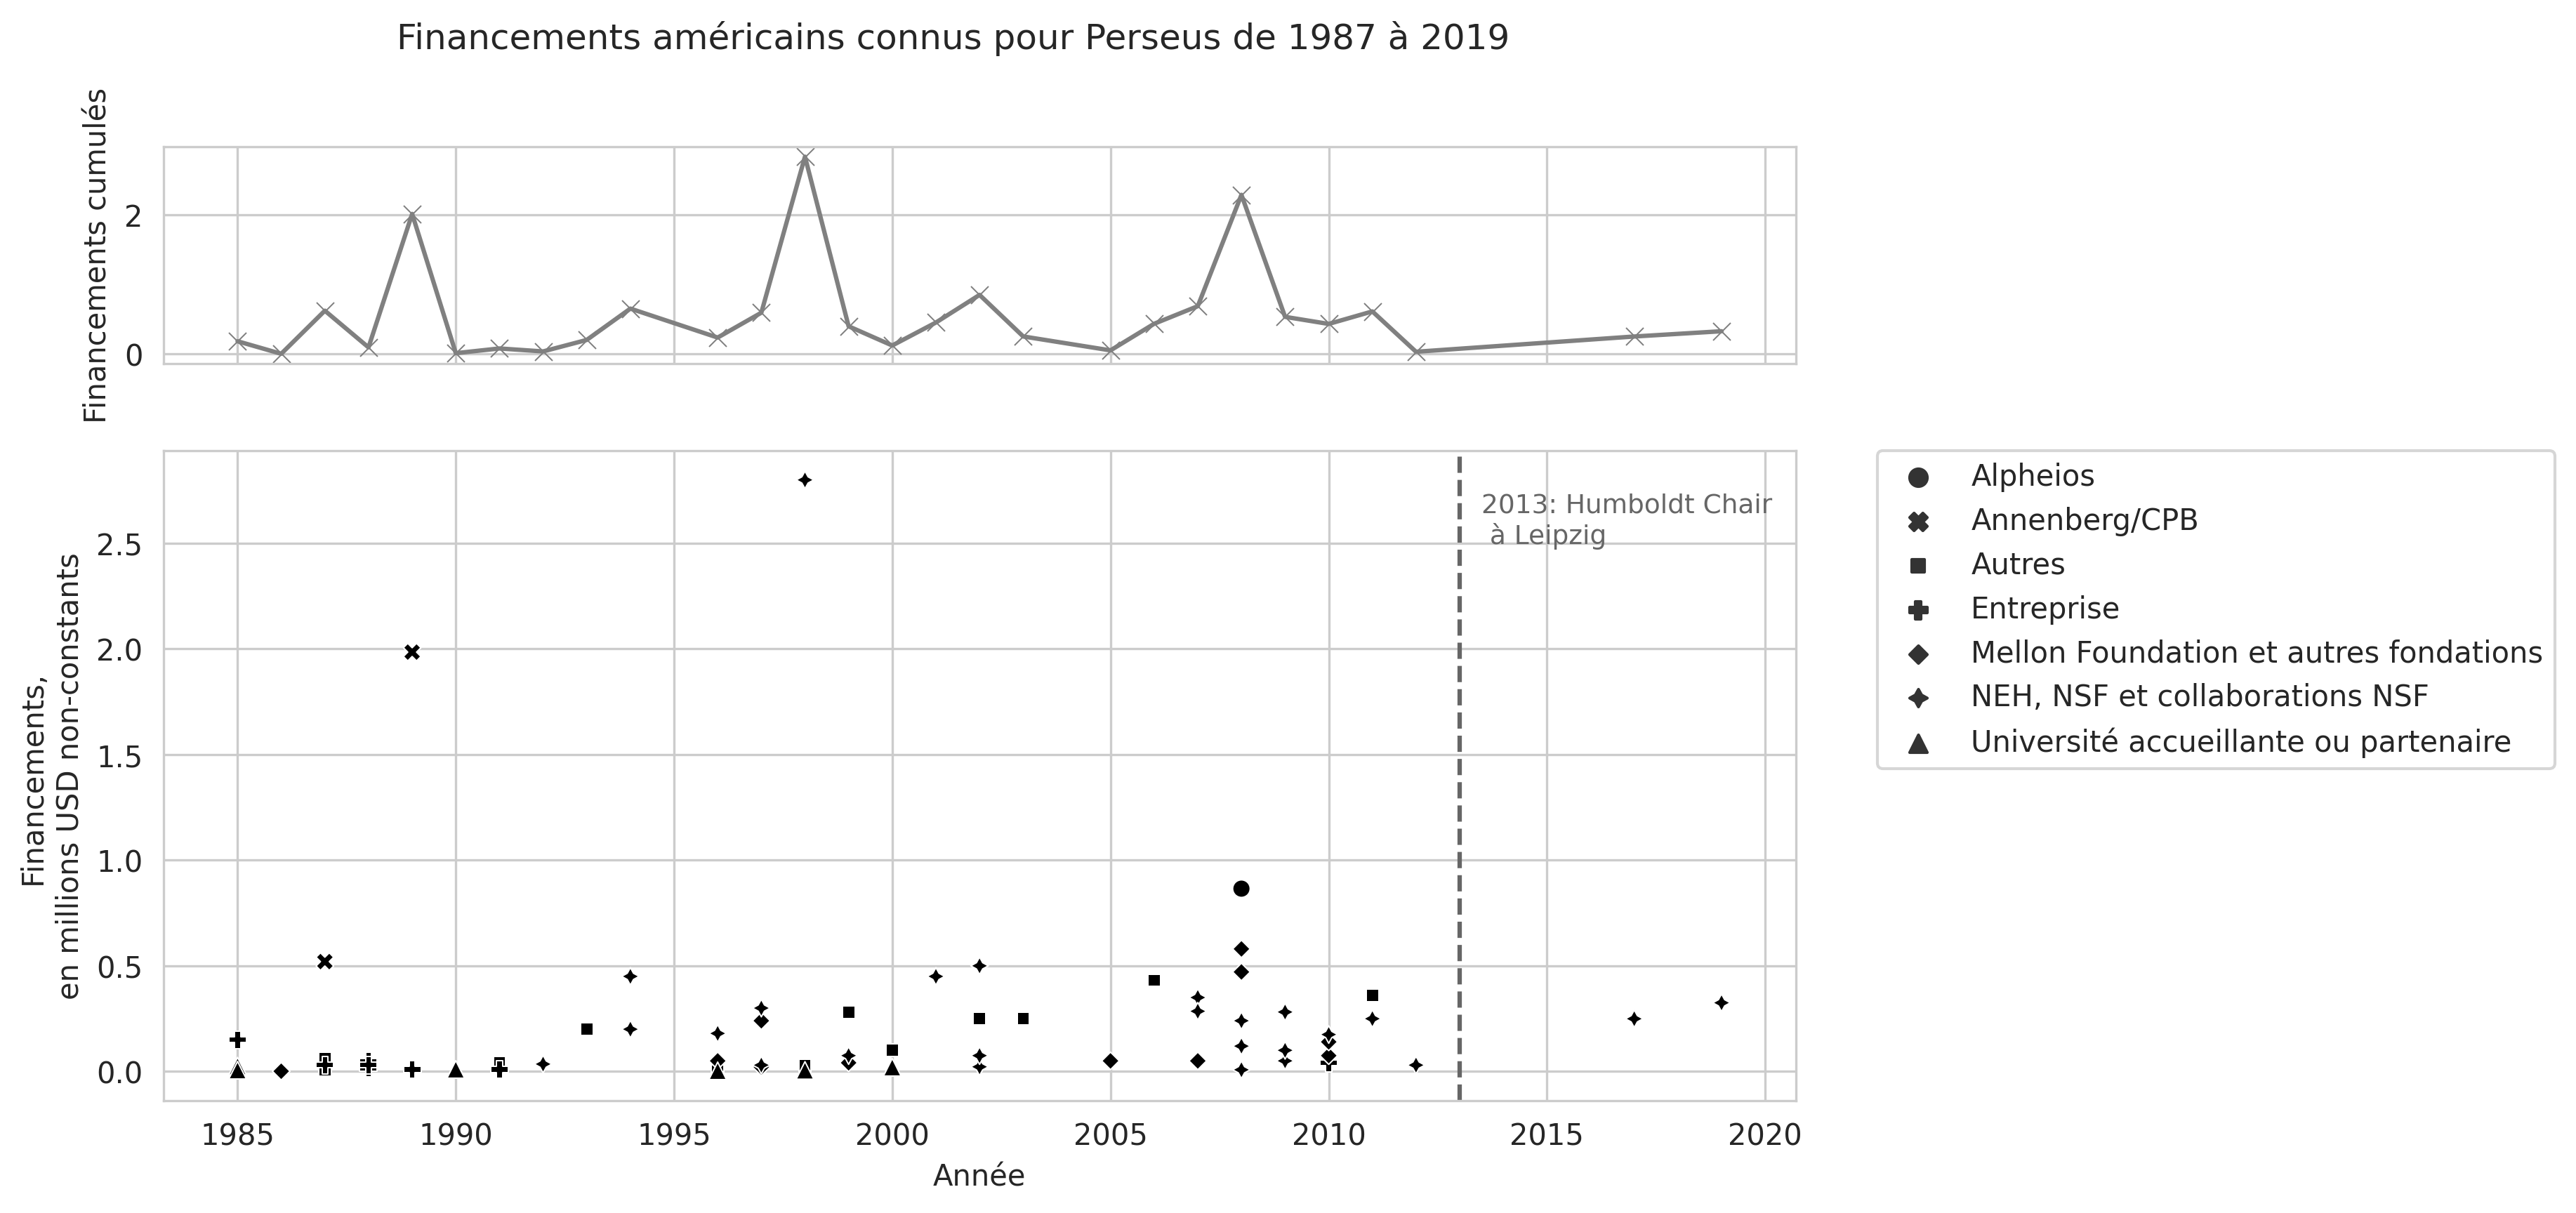
\includegraphics[width=\linewidth]{figures/chap1/part1/PerseusFinancements.png}
    \caption{Financements américains connus de Perseus, en millions de dollars non-constants, d'après les page \textit{Grants} de Perseus, et les archives de la Mellon Foundation et de la NEH. On distingue clairement trois vagues (1: fondation, 2: web, 3: expansion) et l'exportation de Perseus vers l'Allemagne pendant quelques années pour un retour après la fin des financements à partir de 2017.}
    \label{fig:chap1:perseus_fundings}
\end{figure}

Au milieu de la décennie 2000, la fin du financement \textit{A Digital Library for the humanities} et un ensemble d'autres financements permettent la sortie d'une nouvelle version majeure\footcite{noauthor_gregory_nodate}, la 4.0. La 3.0 ayant subi de nombreuses modifications via les besoins émergents pour l'ensemble des financements de la seconde phase, son code n'est plus maintenable. La 4.0 est une remise à plat complète du projet Perseus, avec un passage vers le langage Java pour la mise à disposition de son site, le passage au XML pour ses ressources textuelles et la mise à disposition pour la première fois de ses données au téléchargement. Ce changement s'opère en 2005, avec une mise en \textit{creative common} de ses sources en 2006 et de son code en \textit{open-source} en 2007\footcite{rockwell_face_2013}. Cette troisième phase marquée par la 4.0 voit l'expansion de Perseus dans le domaine textuel se confirmer: à partir de 2000, aucun financement ne concerne la partie archéologique ou visuelle de Perseus, tandis que se développent une bibliothèque sur la guerre civile (2003), une extension pour les textes arabes (2006), le traitement des entités nommées (2007) ou de la grammaire grecque par Treebank (2008), etc. Les corpus ont grossi, toujours dans un objectif de mise à disposition des traductions\footnote{Avec comme seule source notre expérience pour le projet Perseus, des statistiques de 500~000 visites sur le site par semaine nous sont parvenues.}. Avec l'obtention de la chaire Humboldt pour les Humanités Numériques à Leipzig, la troisième phase s'éteint, et peu de financements sont obtenus du côté américain, malgré une attache conservée à Tufts.
% Phase 2 de Perseus: Le latin et le reste, version 3.0 puis 4.0

Un phénomène nouveau accompagne cette apparition du web dans les foyers et bibliothèques: la naissance de corpus produits par des non-spécialistes, ce que l'on pourrait qualifier aujourd'hui de \enquote{\textit{citizen sciences} avant l'heure}, c'est-à-dire la mise à disposition par l'effort de particuliers hors système de documents ou données scientifiques. Trois corpus existant encore en 2021 naissent sur la période 1995-1998: \textit{Curculio}\footcite{hendry_curculio_1995}, \textit{LacusCurtius}\footcite{lomarcan_lacuscurtius_1999} et \textit{The Latin Library}\footcite{carey_latin_1998} (1998). Les trois se concentrent en particulier sur la problèmatique des textes latins, et pour cause, ni Perseus ni PHI ne fournissent alors ces corpus. Ils sont rejoints par des projets francophone dans la décennie 2000, qui correspond à l'explosion de l'accès au web en France et en Europe: \textit{Remacle.org} arrive en 2003\footcite{philippe_remacle_site_2008}, \textit{Latin, Grec, Juxta} de Gérard Gréco en 2006\footcite{gerard_greco_latin_2006}. La particularité des sites francophones et de leurs fondateurs tient en leur carrière professionnelle: tous deux sont professeurs de lettres classiques de formation. Quelle que soit la situation professionnelle de l'ensemble de ces créateurs de contenu, ils partagent tous la particularité de réaliser ces projets sans financement propre, en dehors des cadres universitaires, avec parfois une exhaustivité particulièrement importante, comme pour \textit{The Latin Library}, et avec une véritable focalisation sur le latin.

\subsubsection{Les projets nés sur le web}

% Les projets d’éditions
    % Hyperdonat
    % Digital Latin Library

% \subsubsection{ Projets de corpus }

%DigilibLT
%Projets épigraphiques
%Musisque Deoque

\subsubsection{OCR et corpus de masse}

% Méta-corpus
%% Corpus Corporum

% Côté éditorial
% \subsubsection{Le renouveau \textit{Open Greek And Latin} et l’apport de l’OCR de masse}
% Approche Github 
% Approche API ?

% Côté non-éditorial non universitaire et l'hors-classique un peu aussi
% \subsubsection{Les corpus en jachères}
%Archive.org et institutions patrimoniales qui OCRisent
% Réfléxion autour de l'OCR de Archive.org, statistiques obtenues quand on a fait des fouilles

\section{Constituer un corpus de recherche}

\subsection{Constitution d’un corpus général de sources littéraires latines}

\subsubsection{Le choix d’un corpus open-source:Traçabilité des textes, textes et reproductibilité}

% Choix Open-Source uniquement
% Citabilité, manipulabilité, compatibilité: XML-TEI et Capitains

\subsubsection{Méthode d’annotation et de “regroupement”}

% La question de la datation
% Métadonnées de “lecture”: modèles de citation, niveau de citation recommandé (Introduction du concept de SATU ?)

\subsubsection{Les corpus employés et les corpus Lasciva Roma}

% Statistiques sur les corpus Perseus et autres
% La conversion de DigilibLT
% Présentation des corpus Lasciva Roma
%% Priapées
%% Additional-Texts

\subsection{Du corpus au document: qu’est-ce qu’un document pour l’ordinateur ?}

% L’importance du choix de CapiTainS, rerédaction de l’article précédemment écrit

\subsection{Constitution d’un corpus sur l’expression de la sexualité}

\subsubsection{Le choix d’une source: Adams et histoire des tentatives de vocabulaires de la sexualité latine ?}

% TLL et problème du TLL chez Adams

\subsubsection{Conséquence du choix de Adams}

% Les données épigraphiques: pourquoi non.
%% Difficulté de lemmatisation
%% Présence relativement faible

% Les bornes “chronologiques” du corpus
% Notes sur quelques données absentes

\subsubsection{Corpus résultat: format, métadonnées, limites}

% Format et tags: interprétation


\section{Composition et analyse des corpus employés}

\subsection{Analyse de la diversité du corpus par période, auteur et genre}

% Représentativité
% Les périodes creuses ?

\subsection{Analyse du corpus sexuel final (stats et autres)}
% Représentation et sur-représentation des auteurs
%% L’angle mort de l’étude d’Adams: la période Chrétienne sous-représentée ?
% Une analyse lexicométrique du corpus: termes les plus fréquents “hors” stopword ?
% Création d’un corpus négatif:
%% Spécificité des termes du corpus: nombre de termes commun (lemme comme formes, stop-words inclus)
%% Nombre de textes très communs (% de lemmes communs importants) via une analyse à la Tesserae ou autre ?
